\documentclass[11pt,a4paper]{article}
\usepackage[utf8]{inputenc}
\usepackage[T1]{fontenc}
\usepackage{lmodern}
\usepackage[italian]{babel}
\usepackage{amsmath}
\usepackage{amsfonts}
\usepackage{amssymb}
\usepackage{graphicx}
\usepackage{hyperref}
\usepackage{geometry}
\geometry{a4paper, margin=2.5cm}

% Configurazione per il codice Python
\usepackage{listings}
\usepackage{xcolor}
\definecolor{codegreen}{rgb}{0,0.6,0}
\definecolor{codegray}{rgb}{0.5,0.5,0.5}
\definecolor{codepurple}{rgb}{0.58,0,0.82}
\definecolor{backcolour}{rgb}{0.95,0.95,0.92}

\lstdefinestyle{mystyle}{
    backgroundcolor=\color{backcolour},   
    commentstyle=\color{codegreen},
    keywordstyle=\color{magenta},
    numberstyle=\tiny\color{codegray},
    stringstyle=\color{codepurple},
    basicstyle=\ttfamily\footnotesize,
    breakatwhitespace=false,         
    breaklines=true,                 
    captionpos=b,                    
    keepspaces=true,                 
    numbers=left,                    
    numbersep=5pt,                  
    showspaces=false,                
    showstringspaces=false,
    showtabs=false,                  
    tabsize=2
}
\lstset{style=mystyle}

\begin{document}

\begin{titlepage}
    \begin{center}
        \vspace*{0.5cm}
        
        
\includegraphics[width=0.85\textwidth]{Immagini/logo_unifi.jpg}
        
        \vspace{4cm}
        
        {\Huge \textbf{Laboratorio di Algoritmi}\par}
        \vspace{0.5cm}
        {\Large Confronto tra implementazioni di un Albero Binario di Ricerca con duplicati\par}
        
        \vfill
        
        {\Large \textbf{Leonardo Carmannini}\par}
        {\large Matricola: 7136659\par}
        
        \vspace{2cm}
    \end{center}
\end{titlepage}
\newpage

\tableofcontents
\newpage

\section{Introduzione}

L'Albero Binario di Ricerca (ABR, o \textit{Binary Search Tree} - BST) rappresenta una delle strutture dati fondamentali nell'ambito dell'informatica per l'organizzazione e la manipolazione efficiente di dati ordinabili. La sua architettura si basa su una regola gerarchica rigorosa: per ogni nodo dell'albero, tutte le chiavi presenti nel sottoalbero sinistro sono minori della chiave del nodo stesso, mentre quelle nel sottoalbero destro sono maggiori. Questa proprietà permette, in condizioni di bilanciamento, di dimezzare lo spazio di ricerca a ogni passo, garantendo tempi di esecuzione logaritmici $O(\log n)$ per le operazioni di ricerca e inserimento.

Tuttavia, un'implementazione standard dell'ABR è ottimizzata per insiemi di chiavi strettamente univoche. La problematica centrale affrontata in questo progetto emerge quando il set di dati di input presenta una forte incidenza di \textbf{chiavi duplicate}. Se un ABR standard viene istruito ad accettare duplicati (ad esempio, inserendoli sistematicamente nel sottoalbero sinistro), la struttura subisce un rapido e grave degrado strutturale. I duplicati generano catene lineari di nodi che sbilanciano profondamente l'albero, trasformandone l'andamento asintotico da logaritmico a lineare $O(n)$, avvicinando il suo comportamento a quello di una lista concatenata.

Per ovviare a questo problema di inefficienza spaziale e temporale, esistono tecniche di compressione dell'informazione all'interno dei nodi. Questa relazione descrive l'implementazione, l'analisi e il confronto prestazionale di tre diverse varianti strutturali di un Albero Binario di Ricerca:

\begin{itemize}
    \item \textbf{ABR Standard (Normale)}: implementazione classica in cui i duplicati vengono allocati come nuovi nodi fisici all'interno dell'albero.
    \item \textbf{ABR con Flag}: struttura potenziata in cui i duplicati non generano nuovi nodi, ma vengono tracciati tramite l'aggiornamento di una variabile booleana (o di un contatore di occorrenze) all'interno del nodo primario.
    \item \textbf{ABR con Liste}: approccio ibrido in cui ogni singolo nodo dell'albero contiene una lista dinamica in cui accodare le chiavi identiche, mantenendo compatta la struttura gerarchica dell'albero.
\end{itemize}

\section{Obiettivi dell'attività}

L'obiettivo centrale di questa attività di laboratorio è validare sperimentalmente come la gestione delle chiavi duplicate influenzi le prestazioni e la struttura di un Albero Binario di Ricerca. Attraverso una fase di test intensiva, si intendono misurare le performance delle operazioni fondamentali (inserimento e ricerca, suddivisa in successo e fallimento) e l'evoluzione dell'altezza dell'albero, lavorando su set di dati di dimensioni crescenti e con percentuali variabili di duplicati (10\%, 50\% e 80\%).

Nello specifico, lo scopo di questo progetto è articolato in tre punti cardine:

\begin{enumerate}
    \item \textbf{Implementazione}: Sviluppare interamente da zero, senza l'ausilio di librerie di strutture dati predefinite, le tre diverse realizzazioni dell'ABR (Normale, con Flag, con Liste). Questo permette di comprendere a fondo le dinamiche di allocazione dei nodi e di gestione dei puntatori.
    \item \textbf{Sviluppo di un Framework di Test}: Progettare una metodologia di test rigorosa e automatizzata (\texttt{benchmark.py}) per misurare con precisione i tempi di esecuzione e l'altezza strutturale. I test prevedono l'utilizzo di input controllati (campionamento uniforme per la ricerca) e ripetizioni statistiche per mitigare il rumore del sistema operativo.
    \item \textbf{Analisi Critica e Comparativa}: Analizzare i risultati sperimentali ottenuti, confrontandoli sistematicamente con le previsioni della teoria della complessità computazionale. L'obiettivo finale è dimostrare empiricamente come le tecniche di compressione delle chiavi omologhe prevengano la degenerazione dell'albero, mantenendo le prestazioni vicine all'ottimo logaritmico.
\end{enumerate}

\section{Analisi Teorica, Implementazione e Performance Attese}

In questa sezione viene approfondita l'architettura logica delle tre strutture dati implementate, analizzando il comportamento algoritmico delle operazioni fondamentali e le scelte progettuali effettuate in fase di codifica.

\subsection{ABR Standard (Normale)}

Questa variante rappresenta l'implementazione classica e non ottimizzata dell'Albero Binario di Ricerca. 

\subsubsection{Descrizione delle Operazioni}
Nell'implementazione standard, l'operazione di \textbf{Insert} procede ricorsivamente confrontando la chiave da inserire con il nodo corrente. In caso di chiave duplicata, il nostro algoritmo la tratta come strettamente minore (oppure uguale), allocando sistematicamente un nuovo nodo nel sottoalbero sinistro. 
Di conseguenza, l'operazione di \textbf{Search} dovrà attraversare l'intera catena di nodi identici nel caso cerchi chiavi posizionate più in profondità. La complessità, in presenza di un'altissima percentuale di duplicati, degrada dal caso medio $O(\log n)$ al caso pessimo $O(n)$.

\subsubsection{Implementazione Python}
\begin{lstlisting}[language=Python]
class NodeNormal:
    def __init__(self, key):
        self.key = key
        self.left = None
        self.right = None

class ABRNormal:
    # ...
    def _insert_recursive(self, node, key):
        # I duplicati vengono trattati come minori e inseriti a sinistra
        if key <= node.key:
            if node.left is None:
                node.left = NodeNormal(key)
            else:
                self._insert_recursive(node.left, key)
        else:
            if node.right is None:
                node.right = NodeNormal(key)
            else:
                self._insert_recursive(node.right, key)
\end{lstlisting}

\subsection{ABR con Flag / Contatore}

Questa variante mira a comprimere drasticamente lo spazio occupato dai duplicati modificando la struttura interna del nodo.

\subsubsection{Descrizione delle Operazioni}
L'operazione di \textbf{Insert} scende ricorsivamente lungo l'albero. Se incrocia una chiave identica a quella da inserire, invece di allocare un nuovo nodo fisico, si limita a commutare una variabile booleana (\texttt{has\_duplicate = True}). L'impatto sulla memoria per ogni duplicato aggiuntivo è virtualmente zero e il tempo di inserimento (una volta raggiunto il nodo) è $O(1)$. 
Di conseguenza, l'albero non subisce sbilanciamenti indotti dai duplicati: l'operazione di \textbf{Search} per chiavi rare beneficerà di un albero molto più compatto e di altezze ridotte ($O(\log k)$ dove $k$ è il numero di chiavi \textit{uniche}).

\subsubsection{Implementazione Python}
\begin{lstlisting}[language=Python]
class NodeFlag:
    def __init__(self, key):
        self.key = key
        self.left = None
        self.right = None
        self.has_duplicate = False # Flag inizialmente spento

class ABRFlag:
    # ...
    def _insert_recursive(self, node, key):
        # Se la chiave esiste gia', accendiamo solo il flag
        if key == node.key:
            node.has_duplicate = True
        elif key < node.key:
            if node.left is None:
                node.left = NodeFlag(key)
            else:
                self._insert_recursive(node.left, key)
        # ... logica per il sottoalbero destro ...
\end{lstlisting}

\subsection{ABR con Liste di collisione}

Un approccio ibrido che coniuga la struttura ad albero con l'uso di liste concatenate (o array dinamici) all'interno del nodo stesso per collezionare le chiavi omologhe.

\subsubsection{Descrizione delle Operazioni}
Come per l'ABR con Flag, l'\textbf{Insert} non genera nuovi nodi dell'albero quando rileva un duplicato. Invece, accoda il valore (o le eventuali informazioni accessorie) in una lista residente nel nodo (\texttt{self.duplicates.append(key)}). Questo evita lo sbilanciamento gerarchico, ma comporta un leggero overhead computazionale rispetto al semplice flag, dovuto alle operazioni di allocazione dinamica dell'array in Python.

\subsubsection{Implementazione Python}
\begin{lstlisting}[language=Python]
class NodeList:
    def __init__(self, key):
        self.key = key
        self.left = None
        self.right = None
        self.duplicates = [] # Lista per contenere le chiavi omologhe

class ABRList:
    # ...
    def _insert_recursive(self, node, key):
        # Se la chiave esiste gia', accodiamo alla lista interna
        if key == node.key:
            node.duplicates.append(key)
        elif key < node.key:
            if node.left is None:
                node.left = NodeList(key)
            else:
                self._insert_recursive(node.left, key)
        # ... logica per il sottoalbero destro ...
\end{lstlisting}

\subsection{Sintesi delle Complessità Teoriche}

Nella tabella sottostante vengono riassunte le complessità temporali e spaziali asintotiche per le tre implementazioni. L'analisi assume uno scenario critico con una \textbf{fortissima incidenza di duplicati}, evidenziando così il divario prestazionale tra i tre approcci. 

Si definisce $n$ come il numero totale di chiavi (elementi) e $k$ come il numero di chiavi univoche (con $k \ll n$).

\begin{table}[h]
\centering
\renewcommand{\arraystretch}{1.5} % Aumenta il respiro tra le righe per maggiore leggibilita'
\begin{tabular}{|l|c|c|c|}
\hline
\textbf{Struttura Dati} & \textbf{Tempo di Inserimento} & \textbf{Tempo di Ricerca} & \textbf{Spazio di Memoria} \\
\hline
\textbf{ABR Standard} & $O(n)$ & $O(n)$ & $O(n)$ nodi completi \\
\textbf{ABR con Flag} & $O(\log k)$ & $O(\log k)$ & $O(k)$ nodi + $1$ bit per nodo \\
\textbf{ABR con Liste} & $O(\log k)$ & $O(\log k)$ & $O(k)$ nodi + array di taglia $n$ \\
\hline
\end{tabular}
\caption{Confronto delle complessità (temporali e spaziali) in scenari ad alta densità di duplicati.}
\label{tab:complessita}
\end{table}

\section{Metodologia di Testing}

Per garantire l'obiettività e la riproducibilità dei risultati, il processo di benchmark è stato interamente automatizzato attraverso lo script \texttt{benchmark.py}. La metodologia è stata progettata per isolare il comportamento delle strutture dati dalle fluttuazioni casuali del sistema operativo, simulando scenari di utilizzo reali.

\subsection{Protocollo Sperimentale}

Il benchmark segue un protocollo rigoroso basato su set di dati crescenti e misurazioni ripetute:
\begin{itemize}
    \item \textbf{Campionamento Variabile (Dimensioni):} Le strutture sono state testate per valori di $N \in \{500, 1000, 2000, 3000, 5000, 7500, 10000\}$. Questa progressione permette di osservare chiaramente l'emergere delle complessità asintotiche.
    \item \textbf{Incidenza dei Duplicati:} Ogni dimensione è stata testata su tre diversi scenari di congestione: 10\% (incidenza bassa), 50\% (media) e 80\% (alta).
    \item \textbf{Riduzione della Varianza:} Per ogni combinazione (dimensione, percentuale), sono state eseguite \textbf{40 ripetizioni} indipendenti. Questo valore è stato scelto come compromesso ottimale tra un tempo di esecuzione complessivo basso e il rigore necessario per l'eliminazione degli errori di misurazione. 
    \item \textbf{Precisione Temporale:} Le misurazioni sono state effettuate tramite la funzione \texttt{time.perf\_counter()}, scelta per la sua risoluzione ad altissima precisione.
\end{itemize}

\subsection{Generazione dei Dati e Setup}

La corretta generazione degli array di test è la parte più critica per non falsare le valutazioni:
\begin{enumerate}
    \item \textbf{Inizializzazione Pulita:} Ad ogni round, l'array di partenza garantisce matematicamente la percentuale di duplicati richiesta estraendo prima le chiavi uniche e popolando i restanti posti con estratti casuali dalle chiavi già scelte. Infine, una chiamata a \texttt{random.shuffle} previene lo sbilanciamento tipico indotto da inserimenti ordinati sequenzialmente.
    \item \textbf{Test di Ricerca (Successo):} Il test seleziona le $N$ chiavi da cercare effettuando un \textit{campionamento uniforme} sull'insieme delle chiavi \textit{uniche}, e non sull'intero array iniziale. Questa scelta simula query esterne imparziali e penalizza correttamente l'ABR Standard, costringendolo a cercare equamente le chiavi non duplicate che esso stesso aveva sepolto in estrema profondità sotto le catene dei duplicati.
    \item \textbf{Test di Ricerca (Fallimento):} Sono state generate chiavi appartenenti al medesimo intervallo del dataset ma rigorosamente \textit{assenti} dall'albero. Questo forza l'algoritmo di ricerca a percorrere per intero i rami interni (sia a destra che a sinistra) cadendo nelle "trappole" generate dalle catene di duplicati, misurando così il reale costo strutturale delle tre implementazioni.
\end{enumerate}

\subsection{Elaborazione e Visualizzazione dei Dati}

Al termine del processo di misurazione, i tempi grezzi accumulati vengono mediati sul numero totale delle iterazioni per isolare l'esatto contributo della singola operazione algoritmica. Tali metriche vengono poi serializzate in un file persistente in formato \texttt{.csv} (\texttt{risultati.csv}). Questa scelta garantisce una netta separazione tra la fase di calcolo intensivo (benchmark) e la successiva fase di analisi.

Il rendering visivo dei risultati è delegato allo script \texttt{plot\_results.py}, il quale si avvale della libreria \texttt{matplotlib}. Per massimizzare la chiarezza espositiva, i dati sono stati rappresentati tramite \textbf{grafici a barre raggruppate}. Ogni figura è strutturata in un layout a tre pannelli affiancati ($1 \times 3$), corrispondenti alle tre densità di duplicati analizzate (10\%, 50\%, 80\%). 

\section{Analisi dei Risultati}

L'analisi dei dati raccolti conferma sperimentalmente le previsioni teoriche. I grafici prodotti evidenziano in modo inequivocabile il degrado prestazionale e strutturale dell'ABR Standard all'aumentare dell'incidenza dei duplicati, in netto contrasto con le varianti ottimizzate (Flag e Liste) che mantengono un'elevata efficienza.

\subsection{Altezza Strutturale}

L'altezza dell'albero rappresenta la metrica più pura per valutare la degenerazione strutturale della struttura dati. 

\begin{figure}[h]
    \centering
    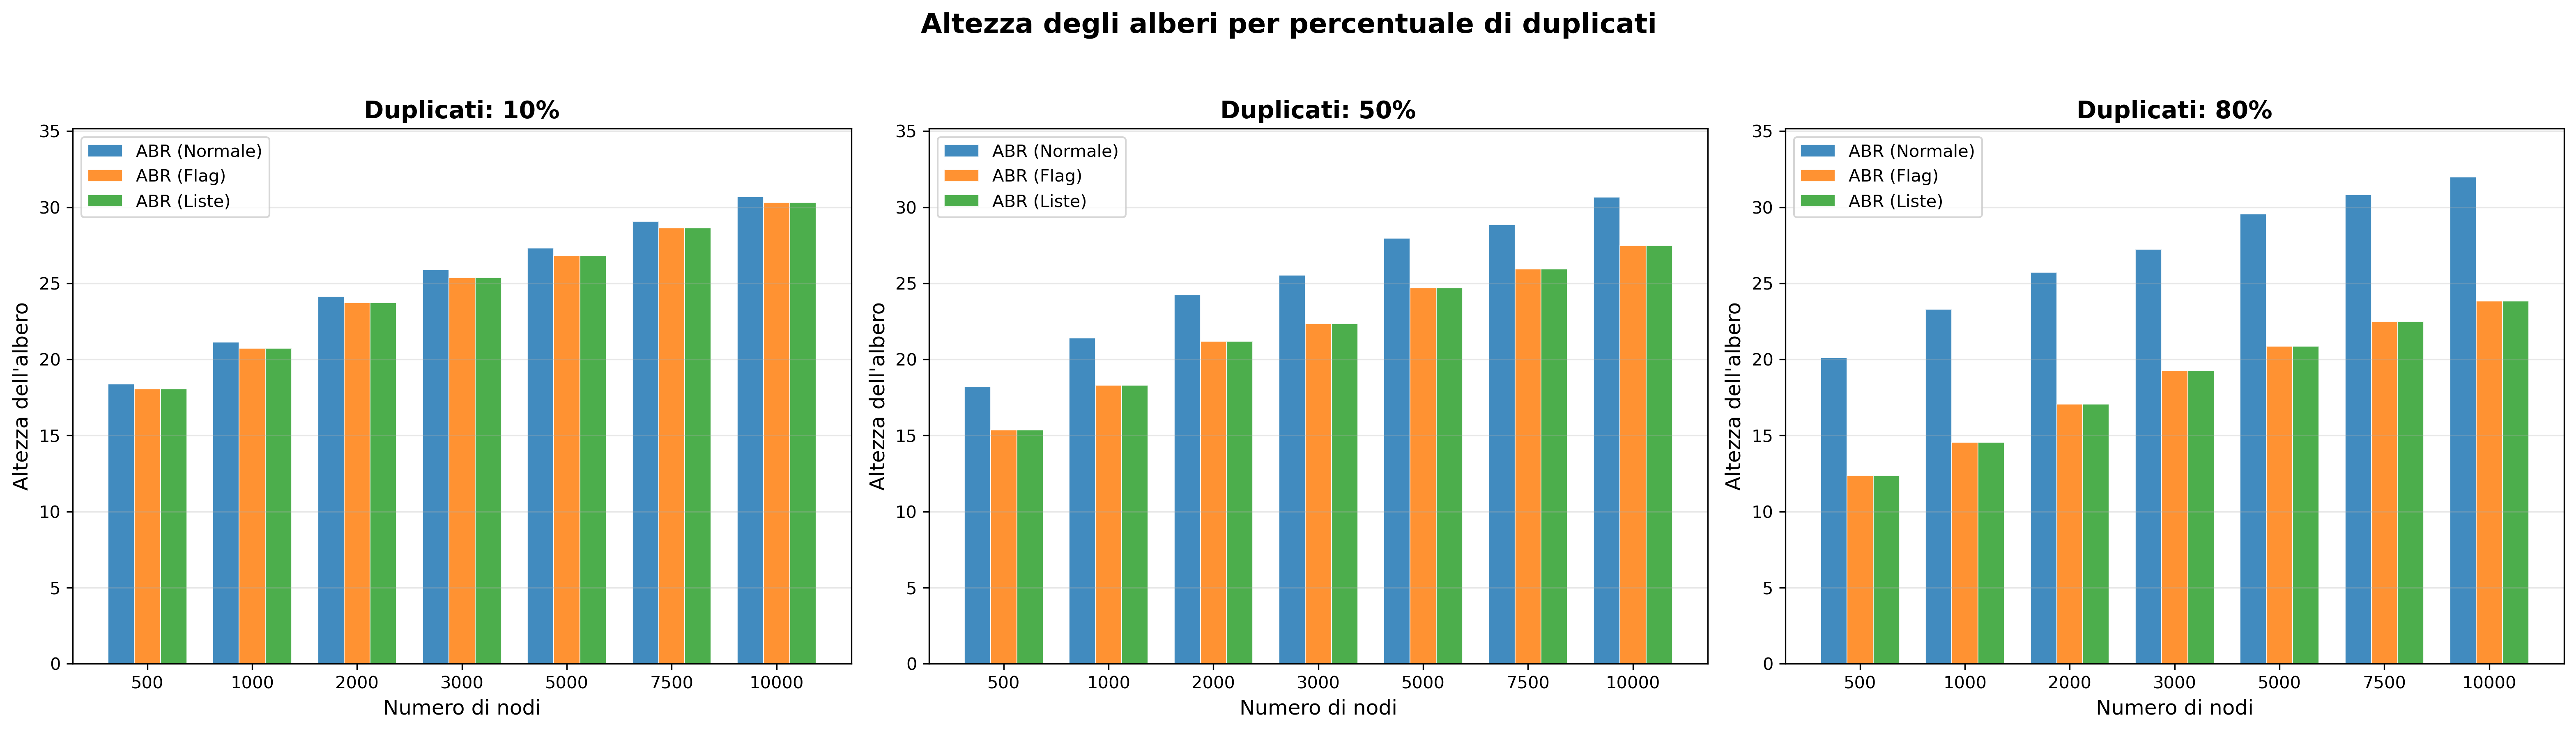
\includegraphics[width=\textwidth]{Immagini/altezza.png}
    \caption{Confronto dell'altezza dell'albero al variare del numero di nodi e della percentuale di duplicati.}
    \label{fig:altezza}
\end{figure}

Dal Grafico \ref{fig:altezza} emerge chiaramente come, al 10\% di duplicati, le tre strutture presentino altezze pressoché identiche. Tuttavia, all'80\% di duplicati, la curva dell'ABR Standard diverge in modo drammatico, crescendo linearmente. Flag e Liste rimangono perfettamente sovrapposte e piatte, poiché la loro altezza dipende unicamente dalle chiavi \textit{uniche}, neutralizzando del tutto il peso dei duplicati.

\subsection{Operazione di Inserimento}

L'operazione di inserimento presenta un interessante trade-off tra il costo computazionale di allocazione in memoria e il costo di attraversamento dell'albero.

\begin{figure}[h]
    \centering
    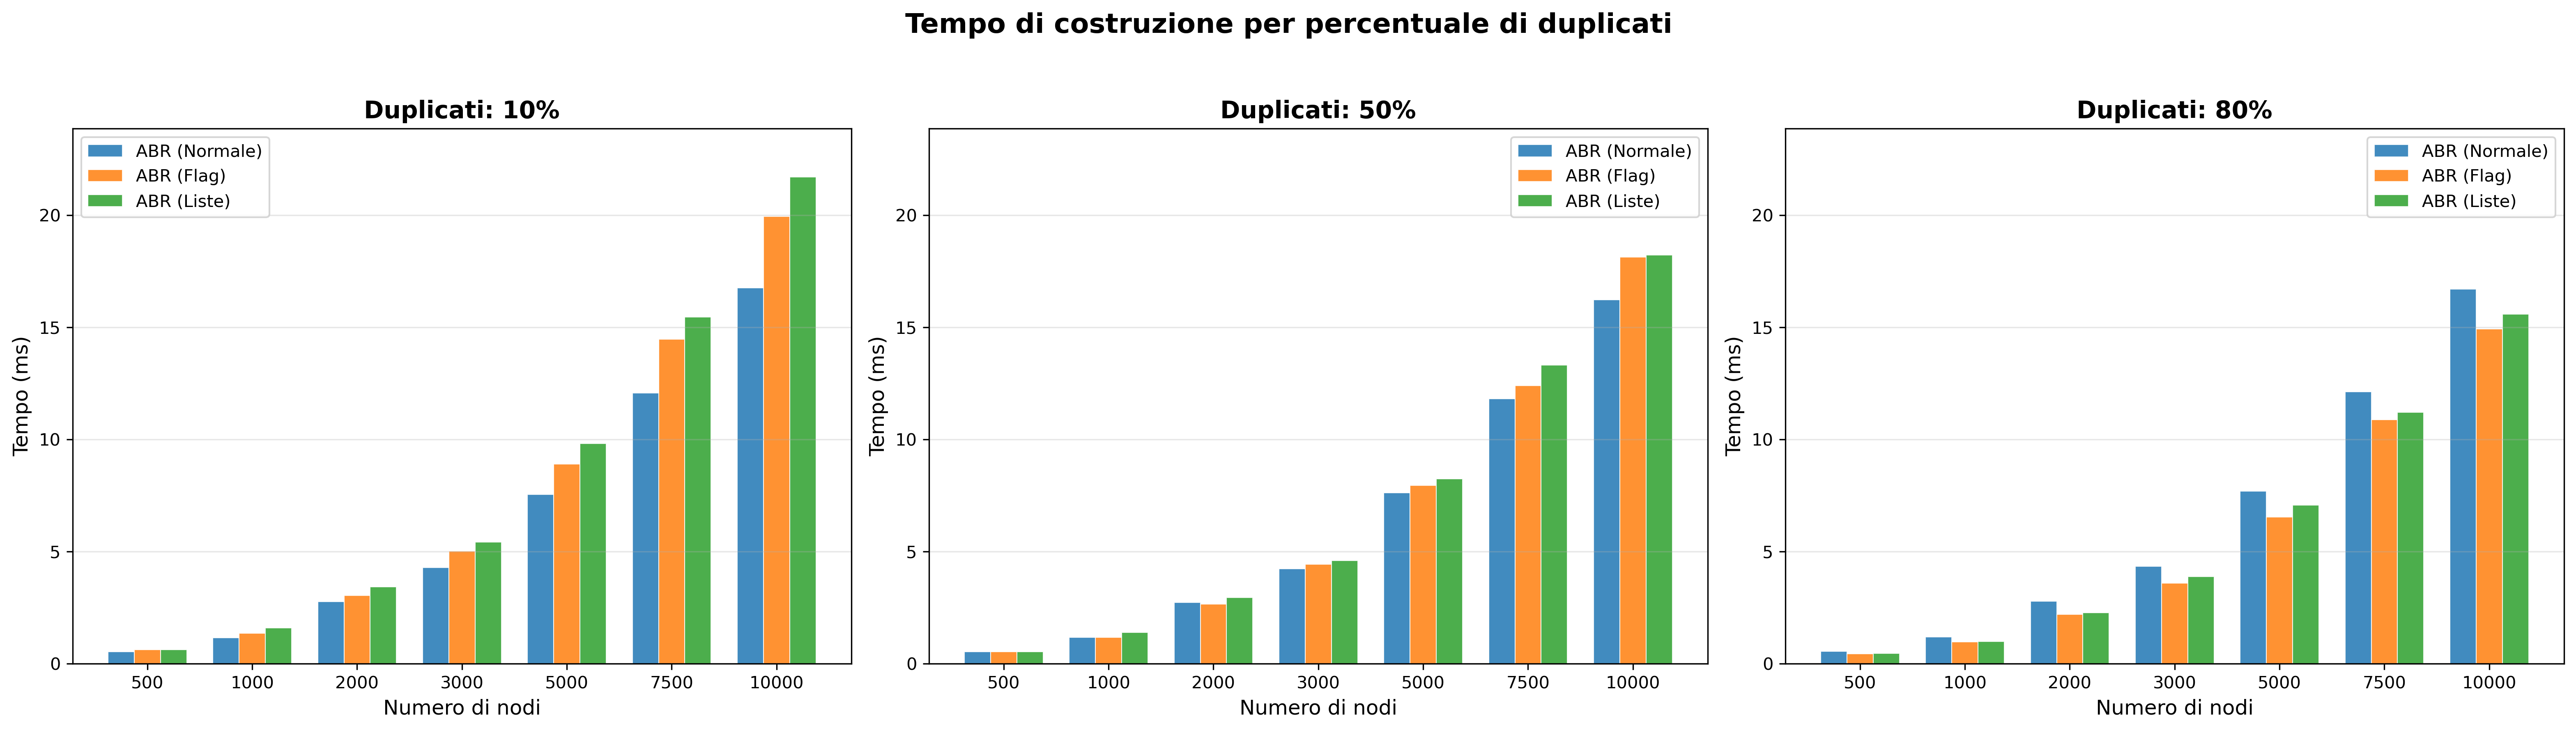
\includegraphics[width=\textwidth]{Immagini/tempi_inserimento.png}
    \caption{Confronto dei tempi medi di inserimento.}
    \label{fig:inserimento}
\end{figure}

Come si evince dal Grafico \ref{fig:inserimento}, al 10\% l'ABR Standard risulta leggermente più rapido: allocare un nodo base è infatti un'operazione meno costosa per l'interprete Python rispetto all'inizializzazione di un array per le Liste. Tuttavia, nello scenario all'80\%, il tempo speso dall'ABR Standard per attraversare le infinite catene di duplicati supera di gran lunga il costo di inizializzazione dei nodi, rendendolo nettamente il più lento tra i tre. L'ABR con Flag si conferma l'approccio più rapido in assoluto in presenza di forti collisioni, richiedendo solo il cambio di stato di un bit ($O(1)$) a struttura già esistente.

\subsection{Operazioni di Ricerca}

I test di ricerca mostrano chiaramente l'efficienza delle strutture compresse.

\begin{figure}[h]
    \centering
    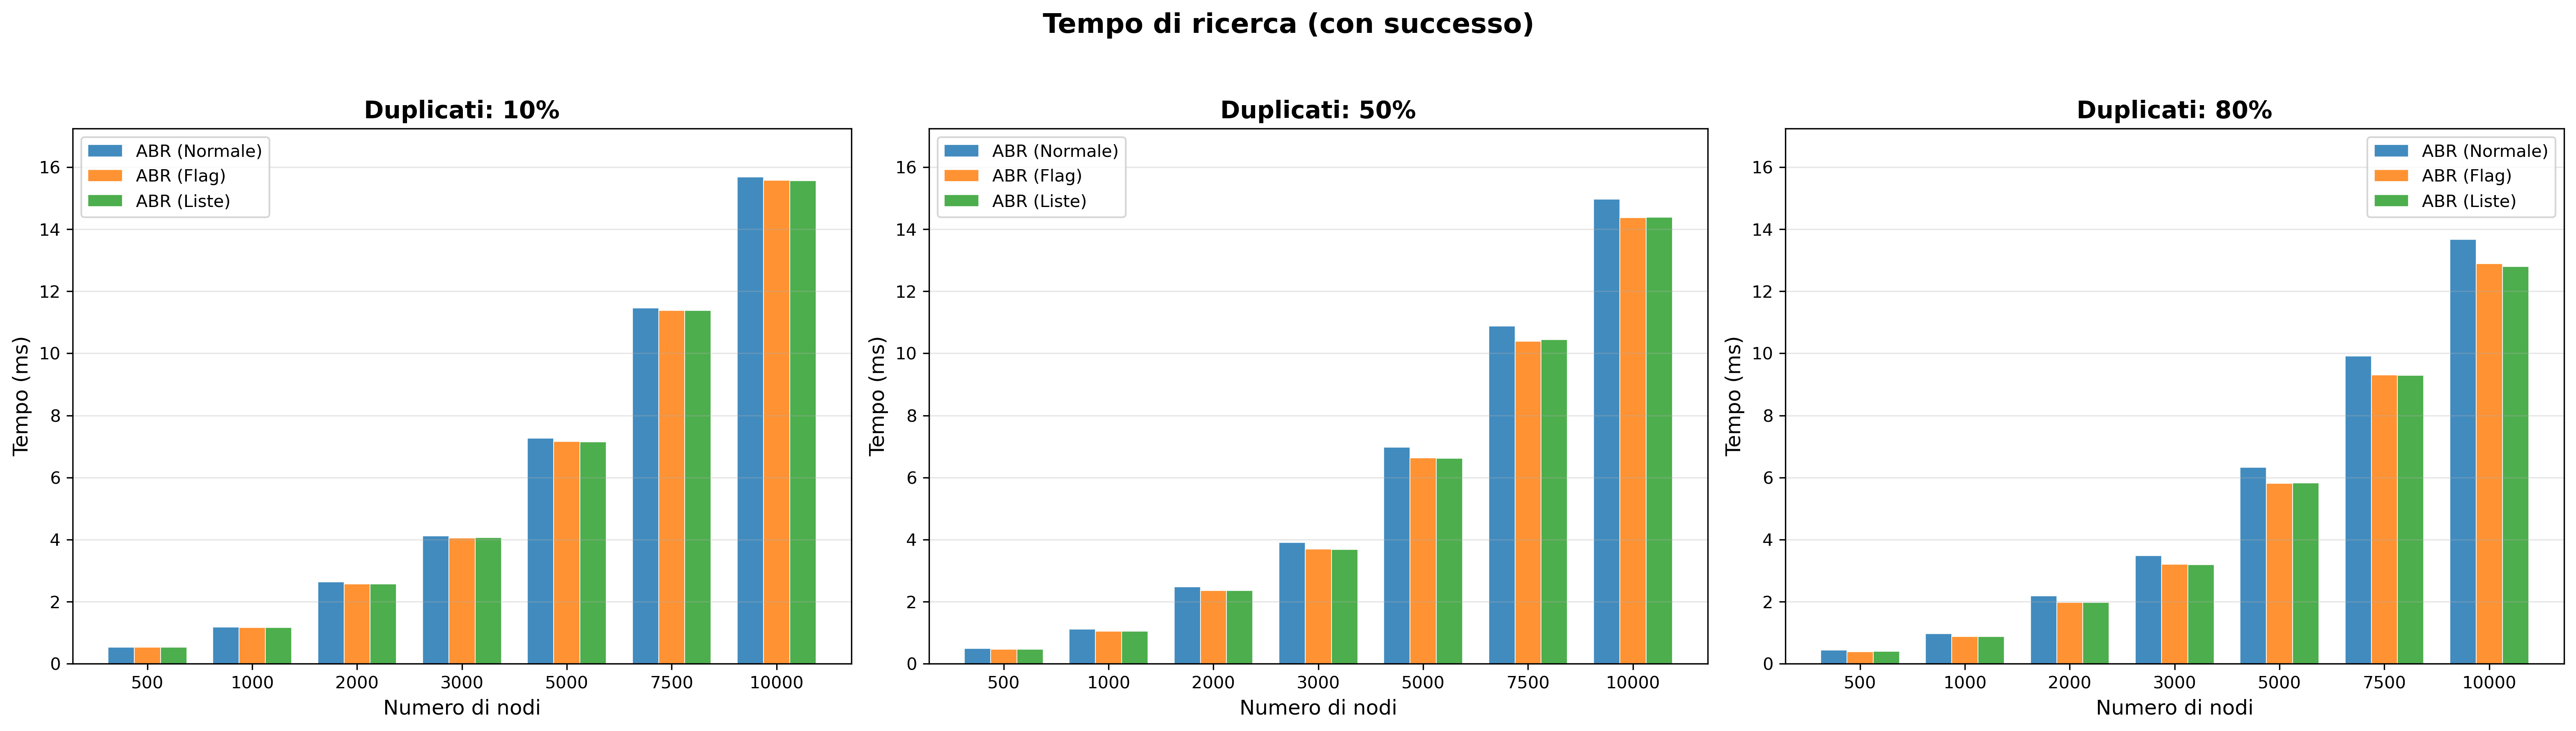
\includegraphics[width=\textwidth]{Immagini/tempi_ricerca_successo.png}
    \caption{Confronto dei tempi medi per la ricerca con successo (campionamento uniforme).}
    \label{fig:ricerca_successo}
\end{figure}

\begin{figure}[h]
    \centering
    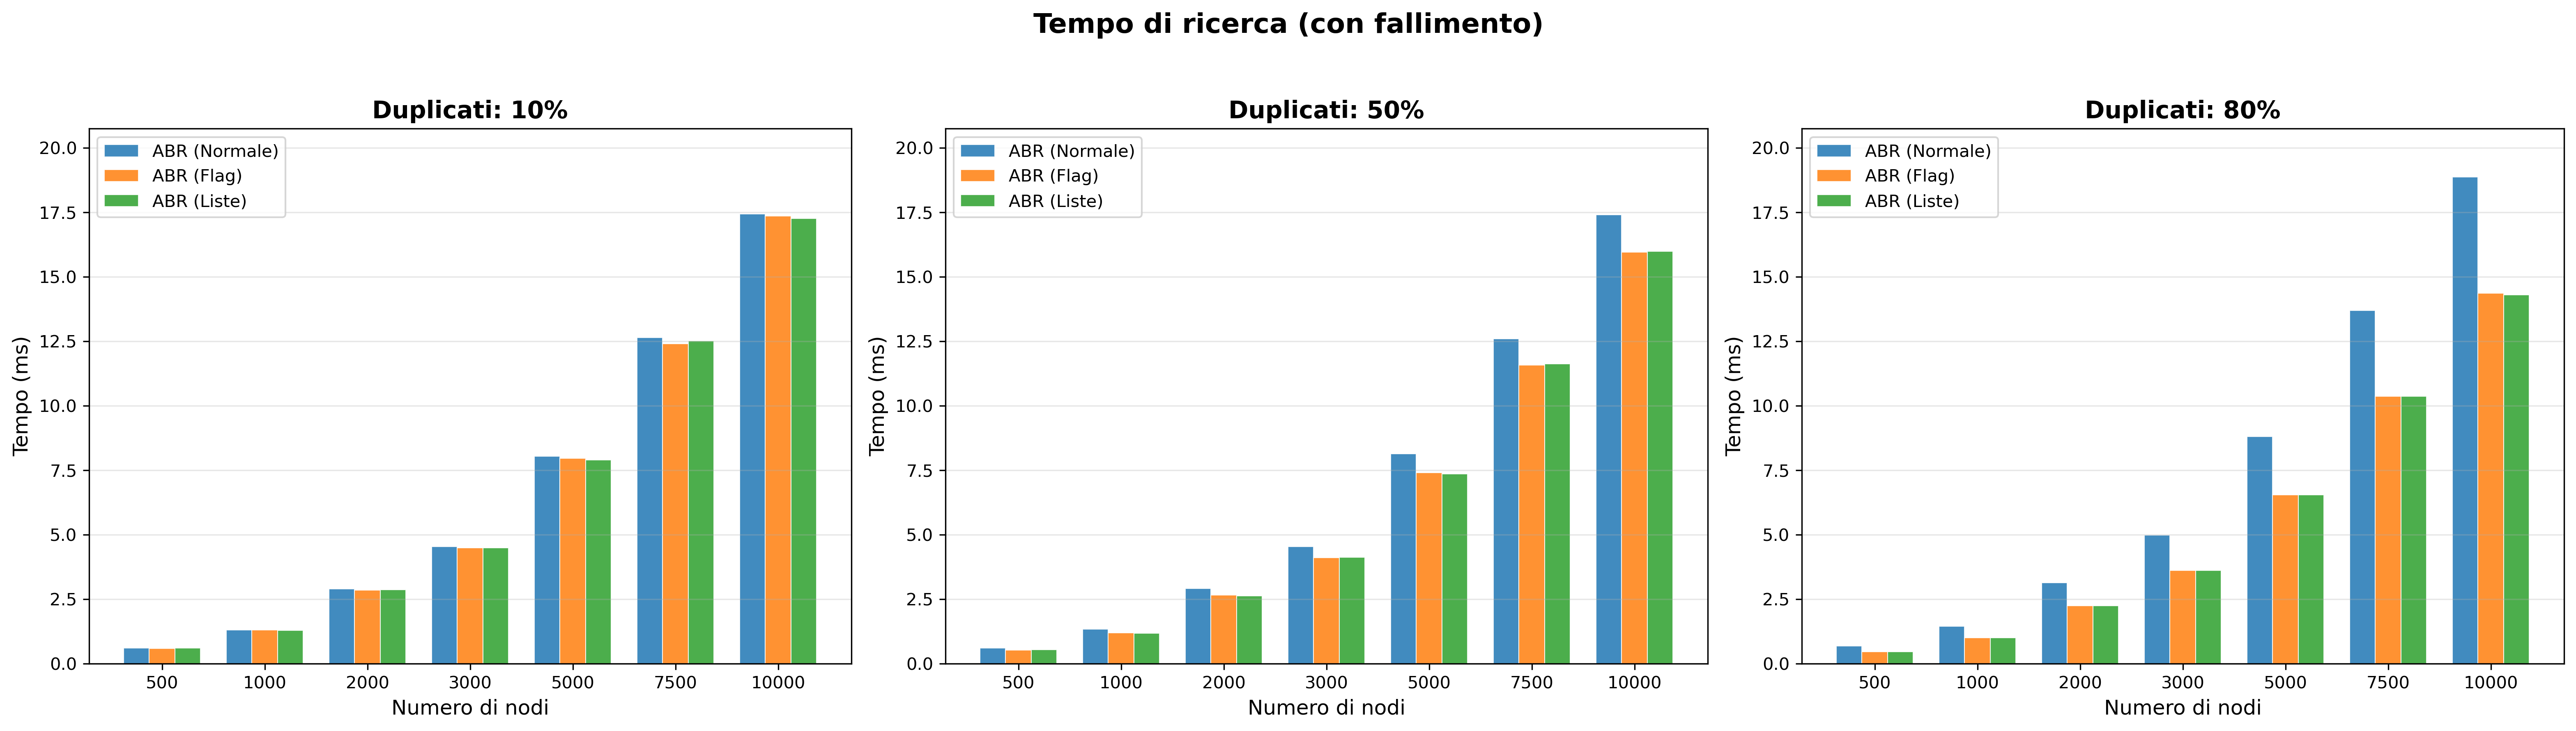
\includegraphics[width=\textwidth]{Immagini/tempi_ricerca_fallimento.png}
    \caption{Confronto dei tempi medi per la ricerca con fallimento (chiavi assenti dal dataset).}
    \label{fig:ricerca_fallimento}
\end{figure}

Nei Grafici \ref{fig:ricerca_successo} e \ref{fig:ricerca_fallimento} è evidente come, oltre la soglia del 50\% di duplicati, la forbice inizi ad allargarsi a sfavore dell'ABR Standard. 
Nello scenario estremo (80\%), l'ABR Standard tocca i tempi massimi. Questo comportamento è la diretta conseguenza dell'altezza eccessiva (come visto in Sezione 5.1): l'algoritmo è costretto a percorrere catene verticali di migliaia di nodi inutili prima di localizzare una chiave "rara" o di dichiarare un fallimento. Flag e Liste, potendo scavalcare l'informazione duplicata in un singolo passaggio, garantiscono tempi di risposta molto più bassi e stabili.

\subsection{Conservazione dell'Informazione e Conteggio Nodi}

Un aspetto cruciale per la scelta implementativa, non catturato unicamente dalle metriche temporali, è il trade-off sulla \textbf{perdita di informazione}. Durante il benchmark, l'operazione ausiliaria di \texttt{conta\_nodi()} ha misurato le istanze fisiche allocate in memoria.

\begin{figure}[h]
    \centering
    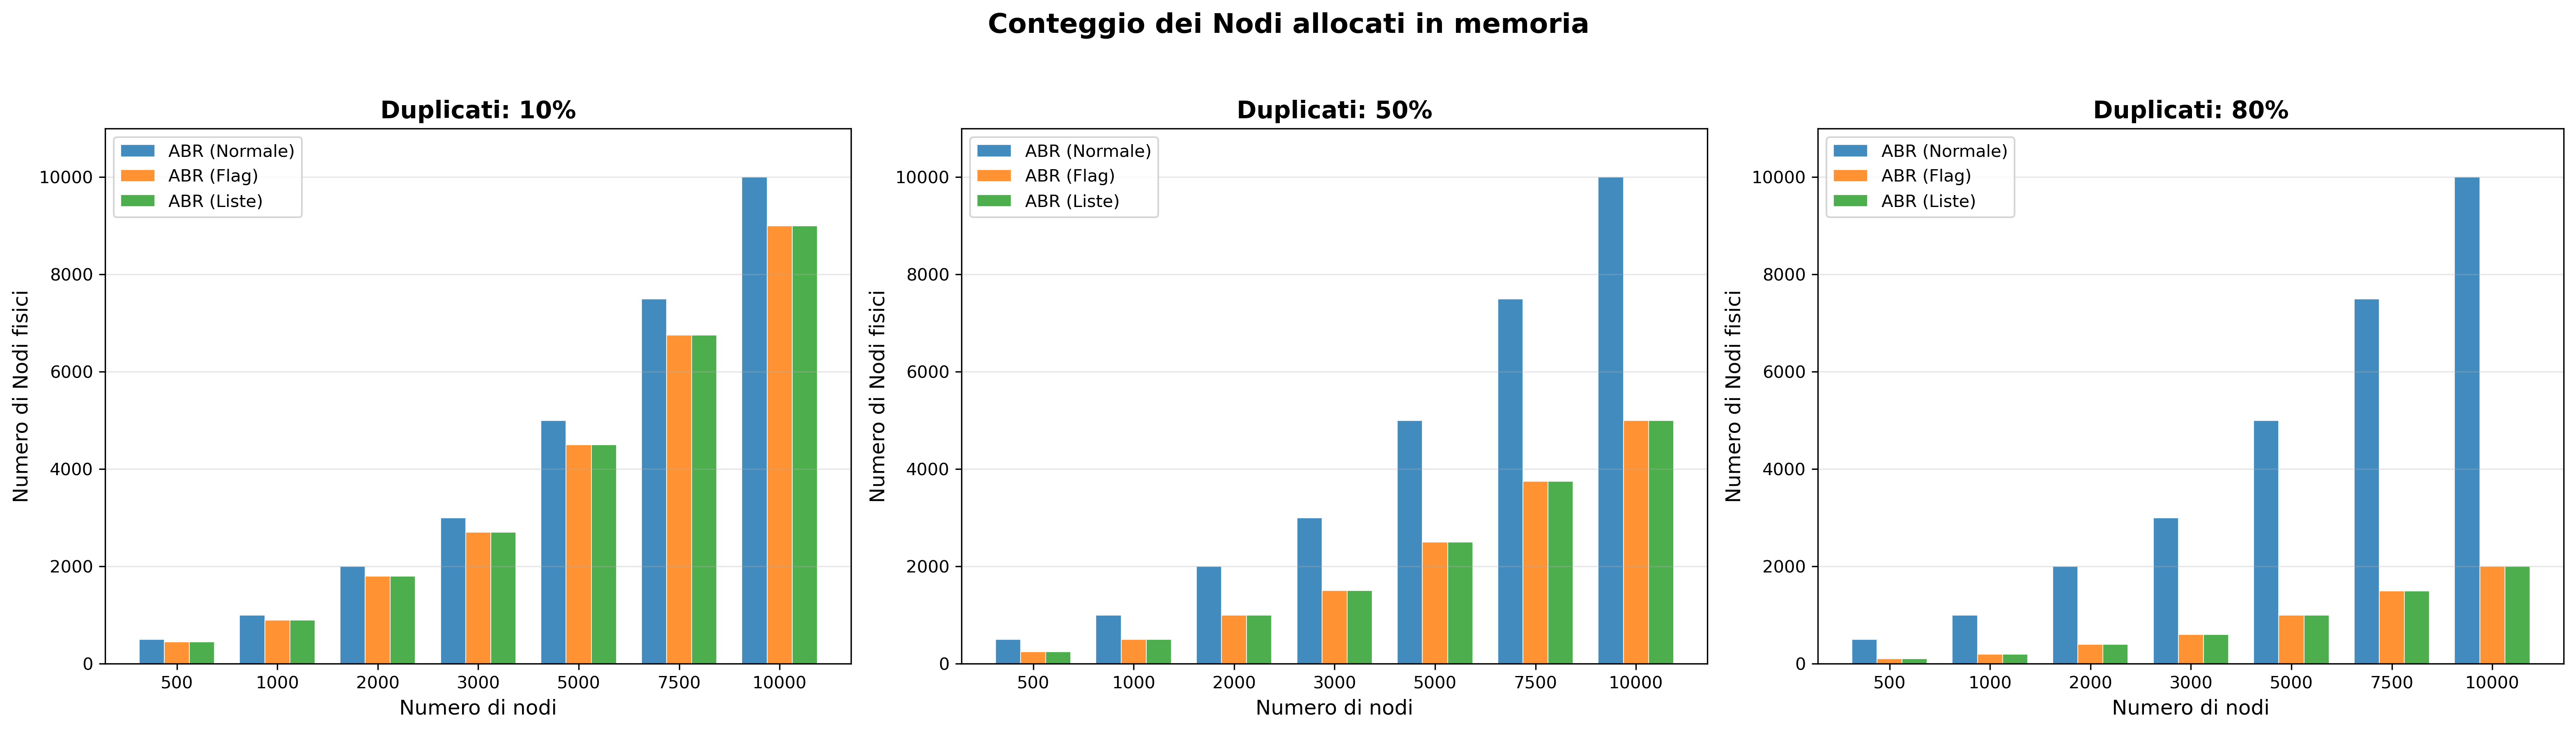
\includegraphics[width=\textwidth]{Immagini/nodi.png}
    \caption{Confronto del numero di nodi fisici allocati in memoria.}
    \label{fig:nodi}
\end{figure}

Dal Grafico \ref{fig:nodi} si evince visivamente quanto teorizzato in precedenza: per l'ABR Standard, i nodi creati coincidono sempre con il numero totale di elementi inseriti ($N$). Per le varianti Flag e Liste, i nodi allocati coincidono esclusivamente con le chiavi \textit{uniche} ($K$). All'80\% di duplicati su 10.000 inserimenti, l'ABR Standard alloca ben 10.000 nodi, mentre Flag e Liste si fermano a circa 2.000 istanze.

Tuttavia, sussiste una profonda differenza semantica tra queste due soluzioni compresse. L'implementazione con \textbf{Flag}, appoggiandosi a un semplice operatore booleano (\texttt{has\_duplicate}), registra unicamente l'\textit{esistenza} di almeno un'omologia. In questo modo si perde irrimediabilmente sia il conteggio esatto delle occorrenze, sia l'eventuale dato satellite (\textit{payload}) associato alla chiave. 
Al contrario, la variante a \textbf{Liste} preserva la totalità del dataset: la lista concatenata interna al nodo conserva in memoria ogni singolo elemento immesso. Questo giustifica il leggero overhead registrato in fase di inserimento (Sezione 5.2), rendendo di fatto la Lista un approccio più "oneroso" ma \textit{lossless} (senza perdita di dati).

\section{Conclusioni}

L'attività di benchmark ha trasformato i modelli teorici in solide evidenze empiriche. L'analisi approfondita dei risultati permette di delineare precisi scenari di utilizzo per ciascuna architettura:
\begin{itemize}
    \item \textbf{ABR Standard}: Si è dimostrato del tutto inadatto a gestire dataset con forti ripetizioni. Il suo impiego in presenza di duplicati porta inevitabilmente a un grave degrado strutturale (catene lineari) e a tempi di risposta asintotici inaccettabili ($O(n)$).
    \item \textbf{ABR con Flag}: È risultata la struttura in assoluto più veloce e compatta in memoria. Rappresenta la scelta ingegneristica ottimale per applicazioni di tipo \textit{Set} (insiemi), dove interessa unicamente tracciare l'esistenza di un elemento e sapere se si è presentata una collisione, accettando la perdita del conteggio esatto e dei dati annessi.
    \item \textbf{ABR con Liste}: Si impone come il miglior compromesso generale. Pur richiedendo uno sforzo allocativo leggermente superiore per istanziare gli array dinamici, è l'unica variante ottimizzata che previene il degrado dell'albero mantenendo intatta la cardinalità e l'integrità del dataset originale. Rappresenta lo standard di riferimento per architetture di tipo \textit{Multimappa} o Dizionario complesso.
\end{itemize}

\end{document}
